\documentclass[11pt, letterpaper, twoside]{article}
\usepackage[utf8]{inputenc}
\usepackage[T1]{fontenc}
\usepackage{fancyhdr}
\usepackage[margin=1in, include foot]{geometry}
\usepackage{ragged2e}
\usepackage[]{hyperref}
\usepackage{apacite}
\usepackage{setspace}
\usepackage{caption}
\usepackage{subcaption}
\usepackage{etoolbox}
\usepackage{graphicx}
\usepackage{amsmath, amssymb}
\usepackage{cleveref}
\usepackage{wrapfig}
\usepackage{afterpage}
\usepackage{floatrow}
\usepackage{tikz}
\usepackage{booktabs}
\usepackage{siunitx}
\usepackage{dcolumn}
\usepackage{pdflscape}
\usepackage{adjustbox}


\setlength{\parindent}{0pt}
\floatsetup[table]{capposition=top}

\title{\singlespacing\textbf{Capture of the Academic Industrial Organization Literature}}


\author{ 
    Joshua Y. Levy \thanks{Joshua Y. Levy  (joshua.levy@chicagobooth.edu), Stigler Center, Booth School of Business, University of Chicago}}
\date{\today}

\onehalfspacing
\begin{document}
\begin{titlepage}
    \maketitle
    \thispagestyle{empty}
\end{titlepage}


\newpage
\pagenumbering{arabic}


\section{The Production of Academic Articles}


% Table created by stargazer v.5.2.3 by Marek Hlavac, Social Policy Institute. E-mail: marek.hlavac at gmail.com
% Date and time: Thu, Apr 28, 2022 - 3:42:28 PM
\begin{table}[!htbp] \centering 
  \caption{} 
  \label{} 
\footnotesize 
\begin{tabular}{@{\extracolsep{5pt}} cccccccc} 
\\[-1.8ex]\hline 
\hline \\[-1.8ex] 
 & AER & ECA & JPE & QJE & RES & RJE & TOTAL \\ 
\hline \\[-1.8ex] 
1990 & $189$ & $66$ & $73$ & $54$ & $42$ & $40$ & $464$ \\ 
1991 & $182$ & $79$ & $67$ & $59$ & $59$ & $41$ & $487$ \\ 
1992 & $196$ & $97$ & $59$ & $56$ & $44$ & $37$ & $489$ \\ 
1993 & $190$ & $54$ & $56$ & $47$ & $48$ & $40$ & $435$ \\ 
1994 & $181$ & $53$ & $54$ & $44$ & $37$ & $36$ & $405$ \\ 
1995 & $174$ & $54$ & $50$ & $41$ & $29$ & $43$ & $391$ \\ 
1996 & $167$ & $58$ & $48$ & $41$ & $28$ & $42$ & $384$ \\ 
1997 & $162$ & $53$ & $54$ & $39$ & $30$ & $48$ & $386$ \\ 
1998 & $174$ & $46$ & $48$ & $42$ & $39$ & $40$ & $389$ \\ 
1999 & $177$ & $87$ & $63$ & $40$ & $42$ & $36$ & $445$ \\ 
2000 & $202$ & $86$ & $52$ & $43$ & $37$ & $35$ & $455$ \\ 
2001 & $201$ & $91$ & $47$ & $42$ & $38$ & $38$ & $457$ \\ 
2002 & $192$ & $116$ & $54$ & $41$ & $39$ & $38$ & $480$ \\ 
2003 & $186$ & $86$ & $47$ & $40$ & $38$ & $42$ & $439$ \\ 
2004 & $189$ & $63$ & $62$ & $41$ & $48$ & $43$ & $446$ \\ 
2005 & $202$ & $57$ & $45$ & $40$ & $46$ & $48$ & $438$ \\ 
2006 & $208$ & $70$ & $39$ & $40$ & $44$ & $59$ & $460$ \\ 
2007 & $214$ & $70$ & $34$ & $44$ & $48$ & $63$ & $473$ \\ 
2008 & $215$ & $70$ & $37$ & $41$ & $51$ & $52$ & $466$ \\ 
2009 & $232$ & $76$ & $32$ & $44$ & $50$ & $35$ & $469$ \\ 
2010 & $257$ & $86$ & $32$ & $44$ & $53$ & $34$ & $506$ \\ 
2011 & $291$ & $70$ & $33$ & $47$ & $50$ & $32$ & $523$ \\ 
2012 & $281$ & $109$ & $30$ & $41$ & $52$ & $32$ & $545$ \\ 
2013 & $260$ & $84$ & $35$ & $56$ & $53$ & $32$ & $520$ \\ 
2014 & $286$ & $89$ & $34$ & $56$ & $52$ & $35$ & $552$ \\ 
2015 & $272$ & $93$ & $37$ & $45$ & $48$ & $36$ & $531$ \\ 
2016 & $286$ & $80$ & $41$ & $40$ & $53$ & $43$ & $543$ \\ 
2017 & $287$ & $89$ & $76$ & $43$ & $57$ & $47$ & $599$ \\ 
2018 & $125$ & $90$ & $85$ & $40$ & $68$ & $40$ & $448$ \\ 
2019 & $139$ & $86$ & $97$ & $41$ & $78$ & $40$ & $481$ \\ 
2020 & $129$ & $116$ & $176$ & $41$ & $81$ & $49$ & $592$ \\ 
2021 & $127$ & $109$ & $101$ & $24$ & $28$ & $11$ & $400$ \\ 
\hline \\[-1.8ex] 
\end{tabular} 
\end{table} 

\begin{figure}
    \begin{subfigure}[!htbp]{0.49\textwidth}
        \centering
        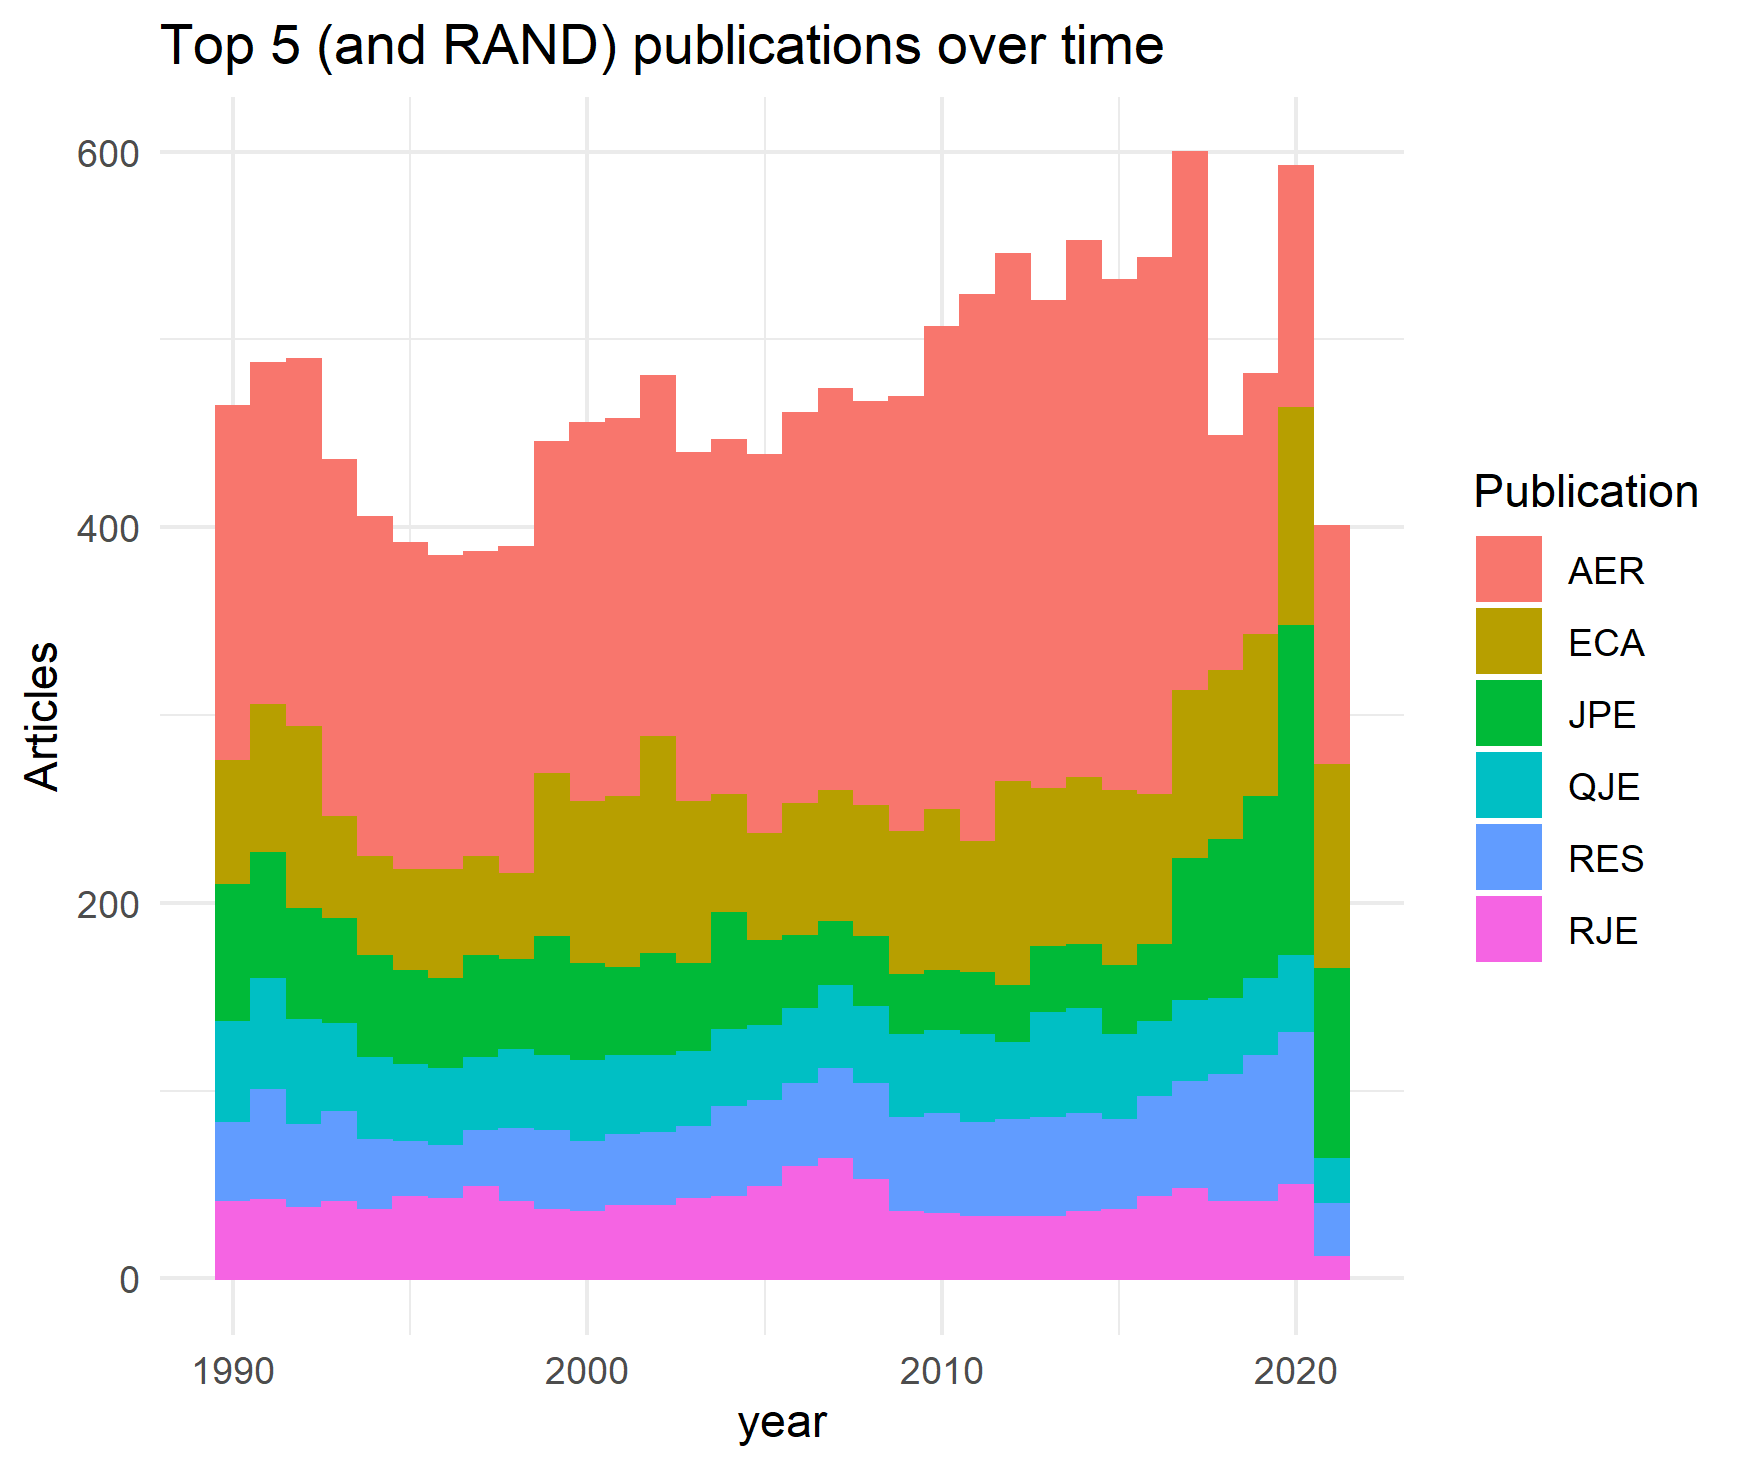
\includegraphics[width=\textwidth]{top_5_over_time_col.png}
        \caption{By count}
    \end{subfigure}
    \hfill
    \begin{subfigure}[!htbp]{0.49\textwidth}
        \centering
        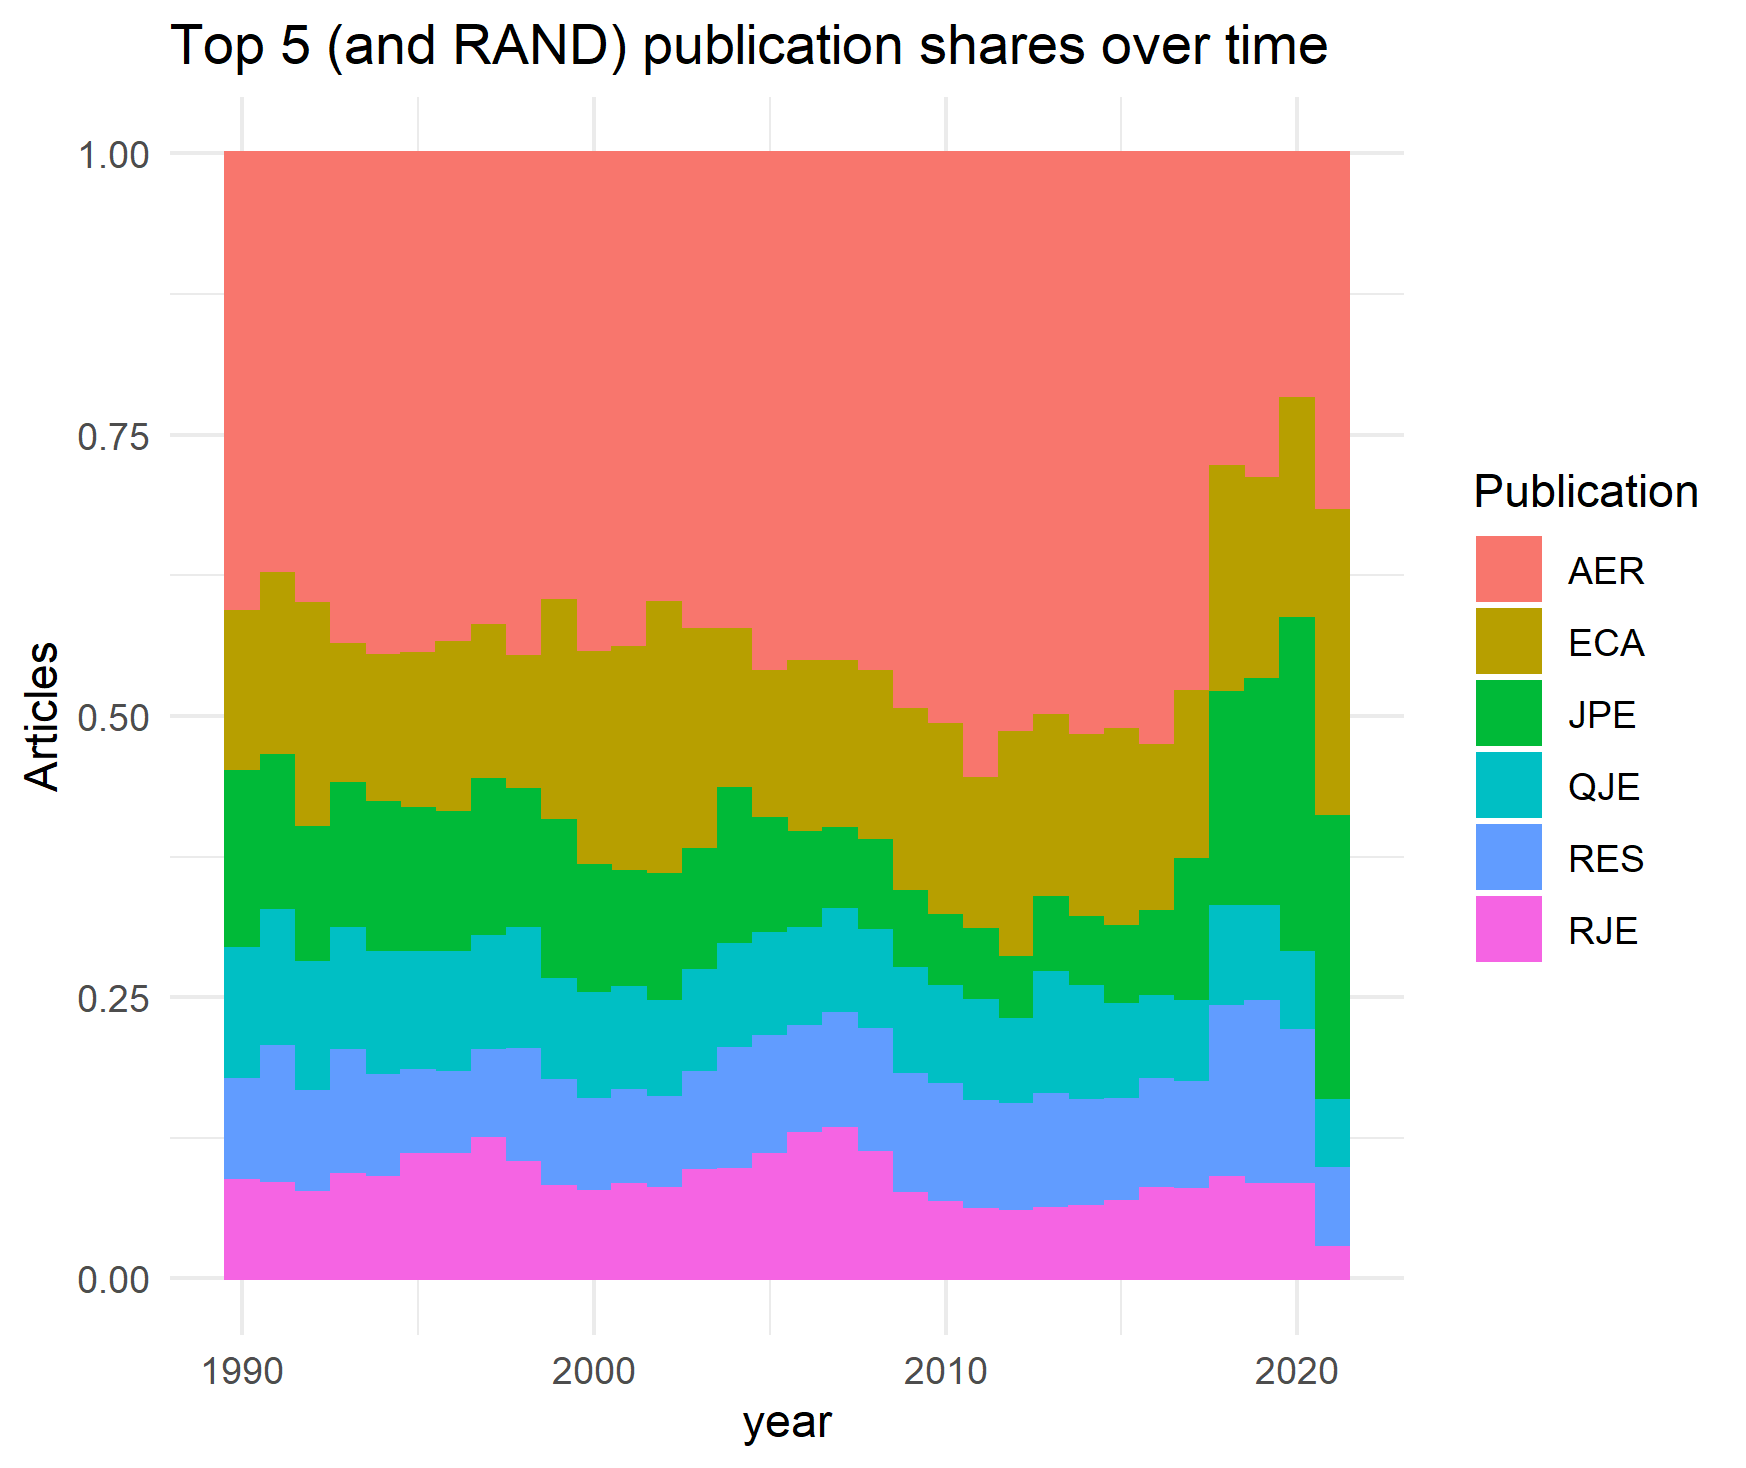
\includegraphics[width=\textwidth]{top_5_over_time_col_shares.png}
        \caption{By share}
    \end{subfigure}
    \begin{subfigure}[!htbp]{\textwidth}
        \centering
        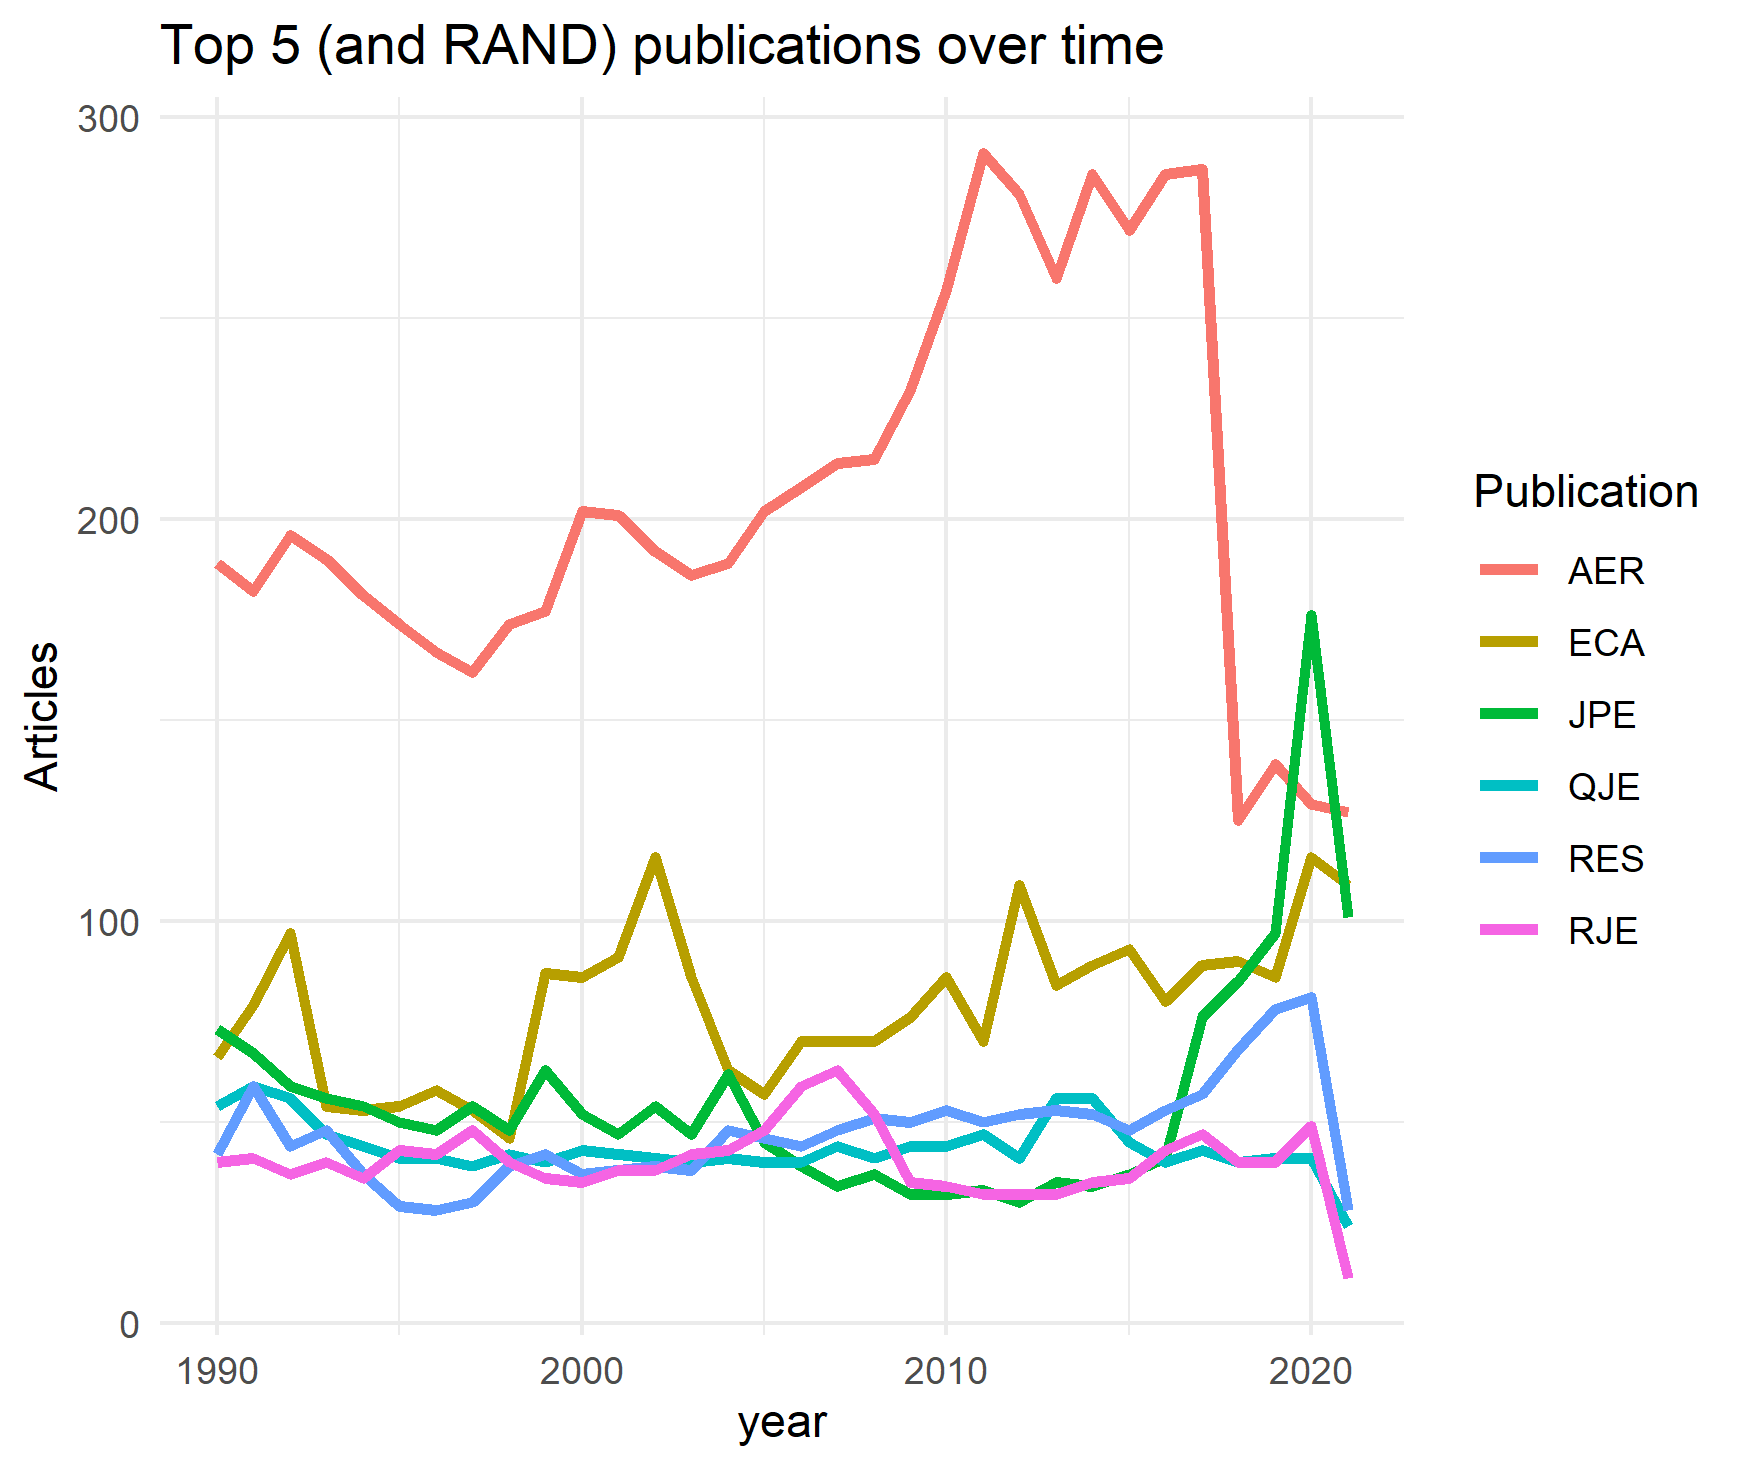
\includegraphics[width=0.5\textwidth]{top5_over_time.png}
        \caption{By count}
    \end{subfigure}
\end{figure}



\section{The Role of Industrial Organization}

These figures use exclusively LXX codes to determine Industrial Organization. (See appendix for more expansive definitions of IO)

\begin{figure}
    \begin{subfigure}[!htbp]{0.49\textwidth}
        \centering
        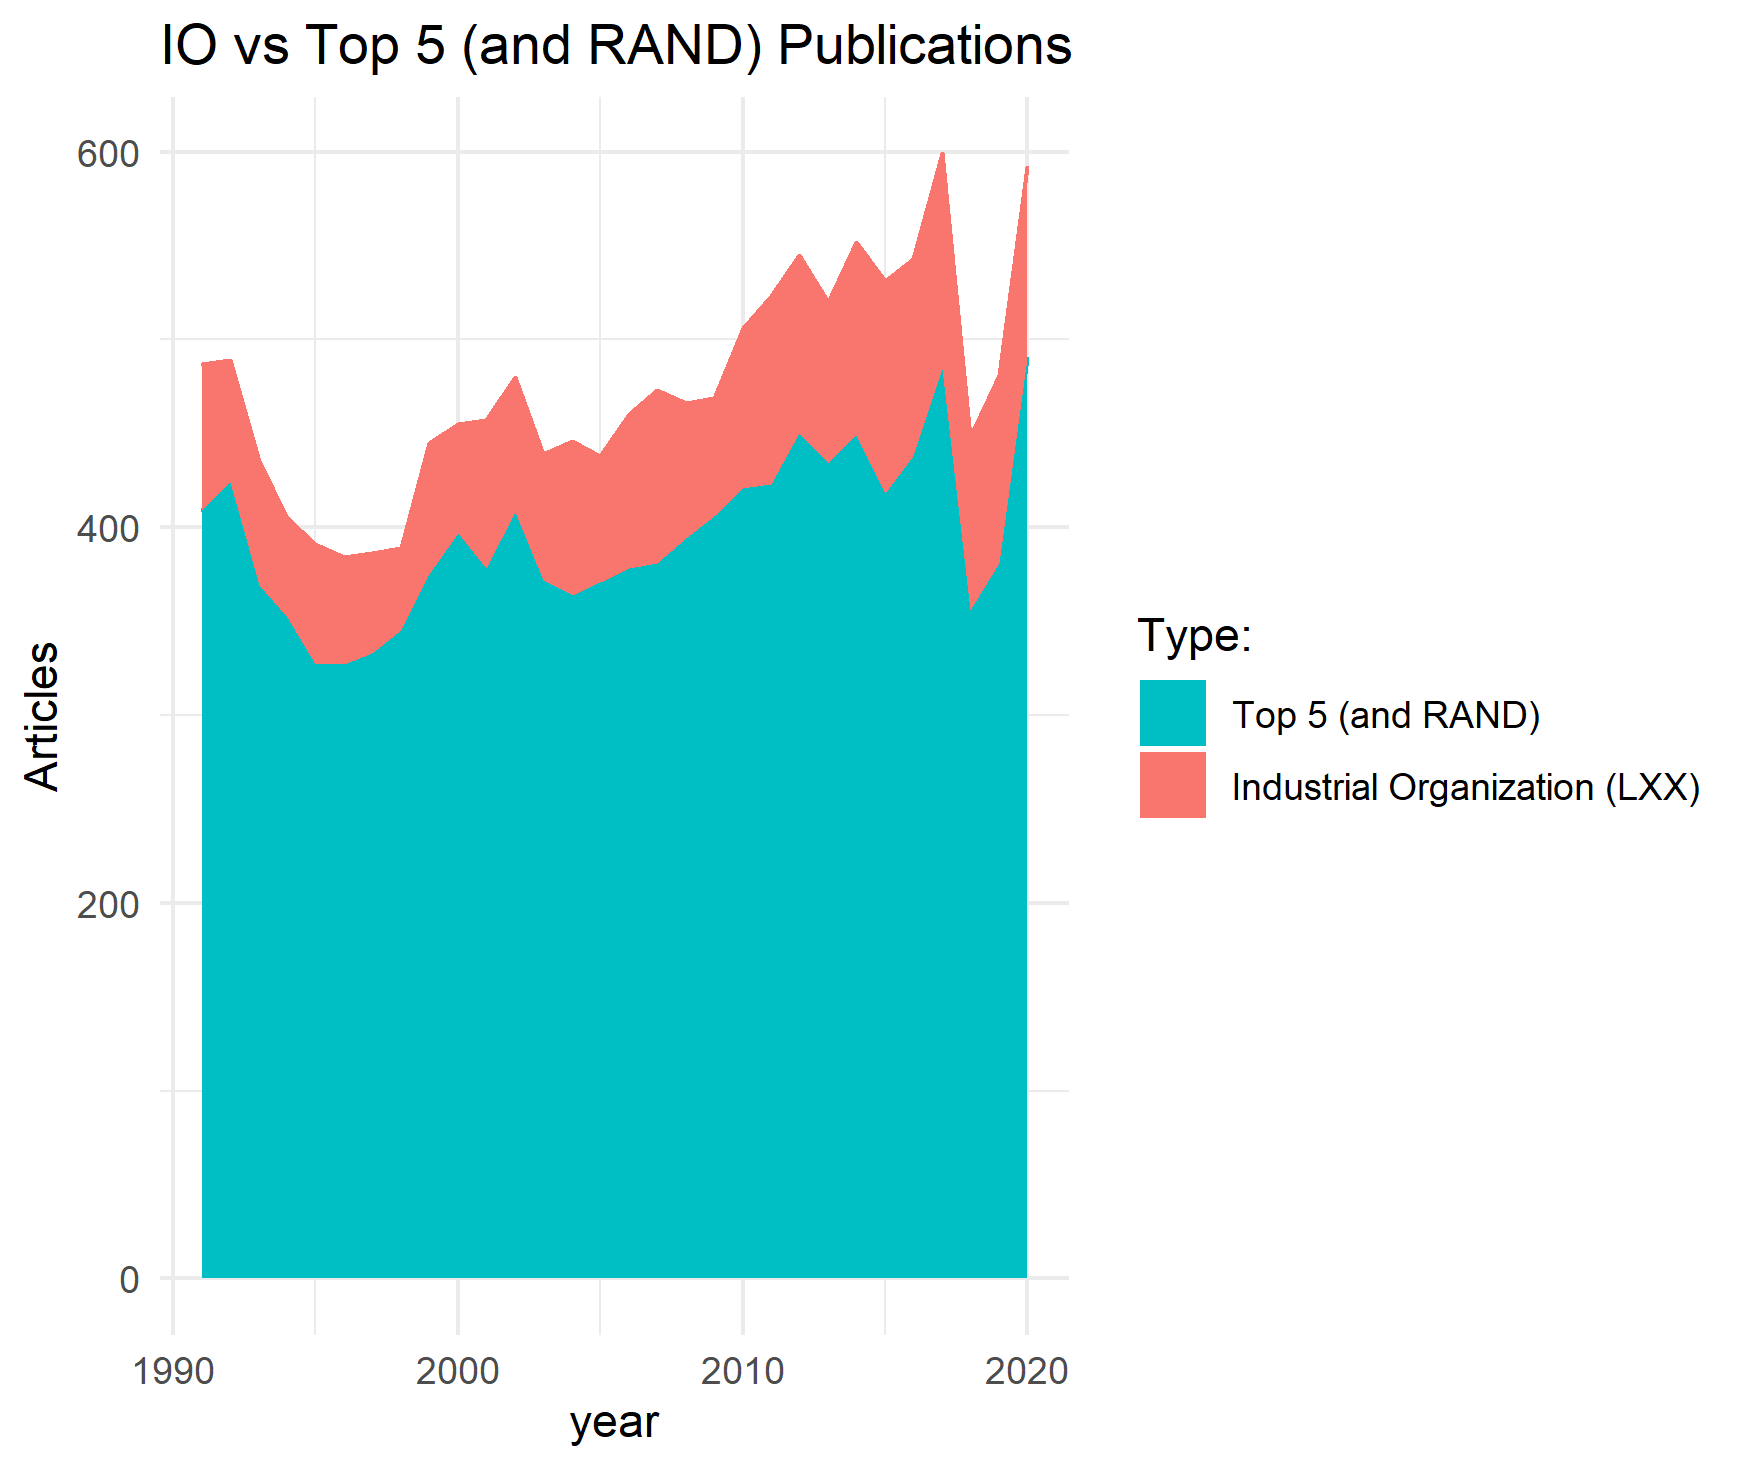
\includegraphics[width=\textwidth]{LXX-code-share-area.png}
    \end{subfigure}
    \hfill
    \begin{subfigure}[!htbp]{0.49\textwidth}
        \centering
        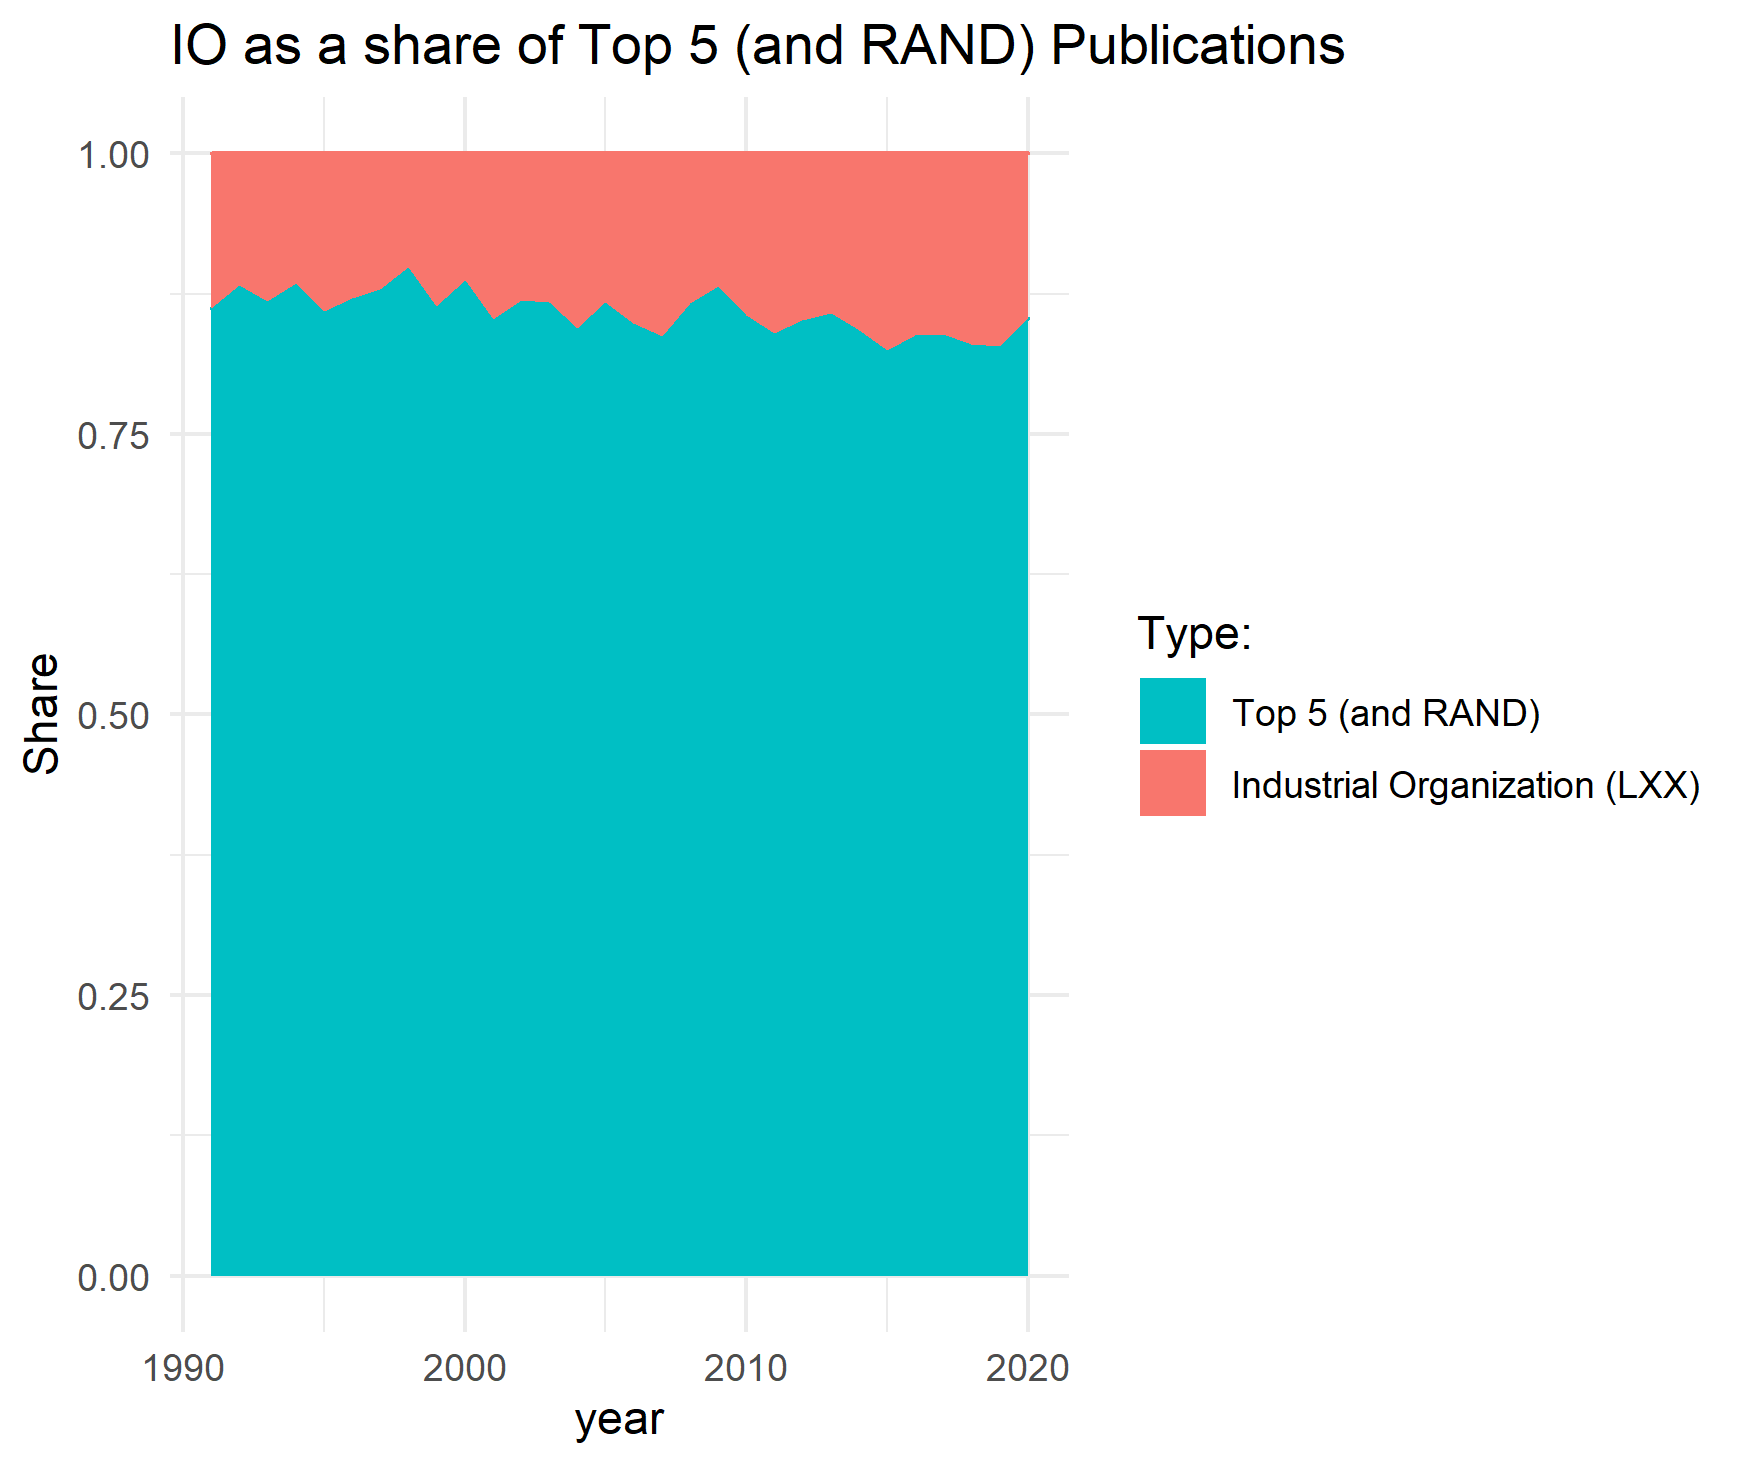
\includegraphics[width=\textwidth]{LXX-code-share-area-normalized.png}
    \end{subfigure}
\end{figure}


\begin{figure}
    \begin{subfigure}[!htbp]{0.49\textwidth}
        \centering
        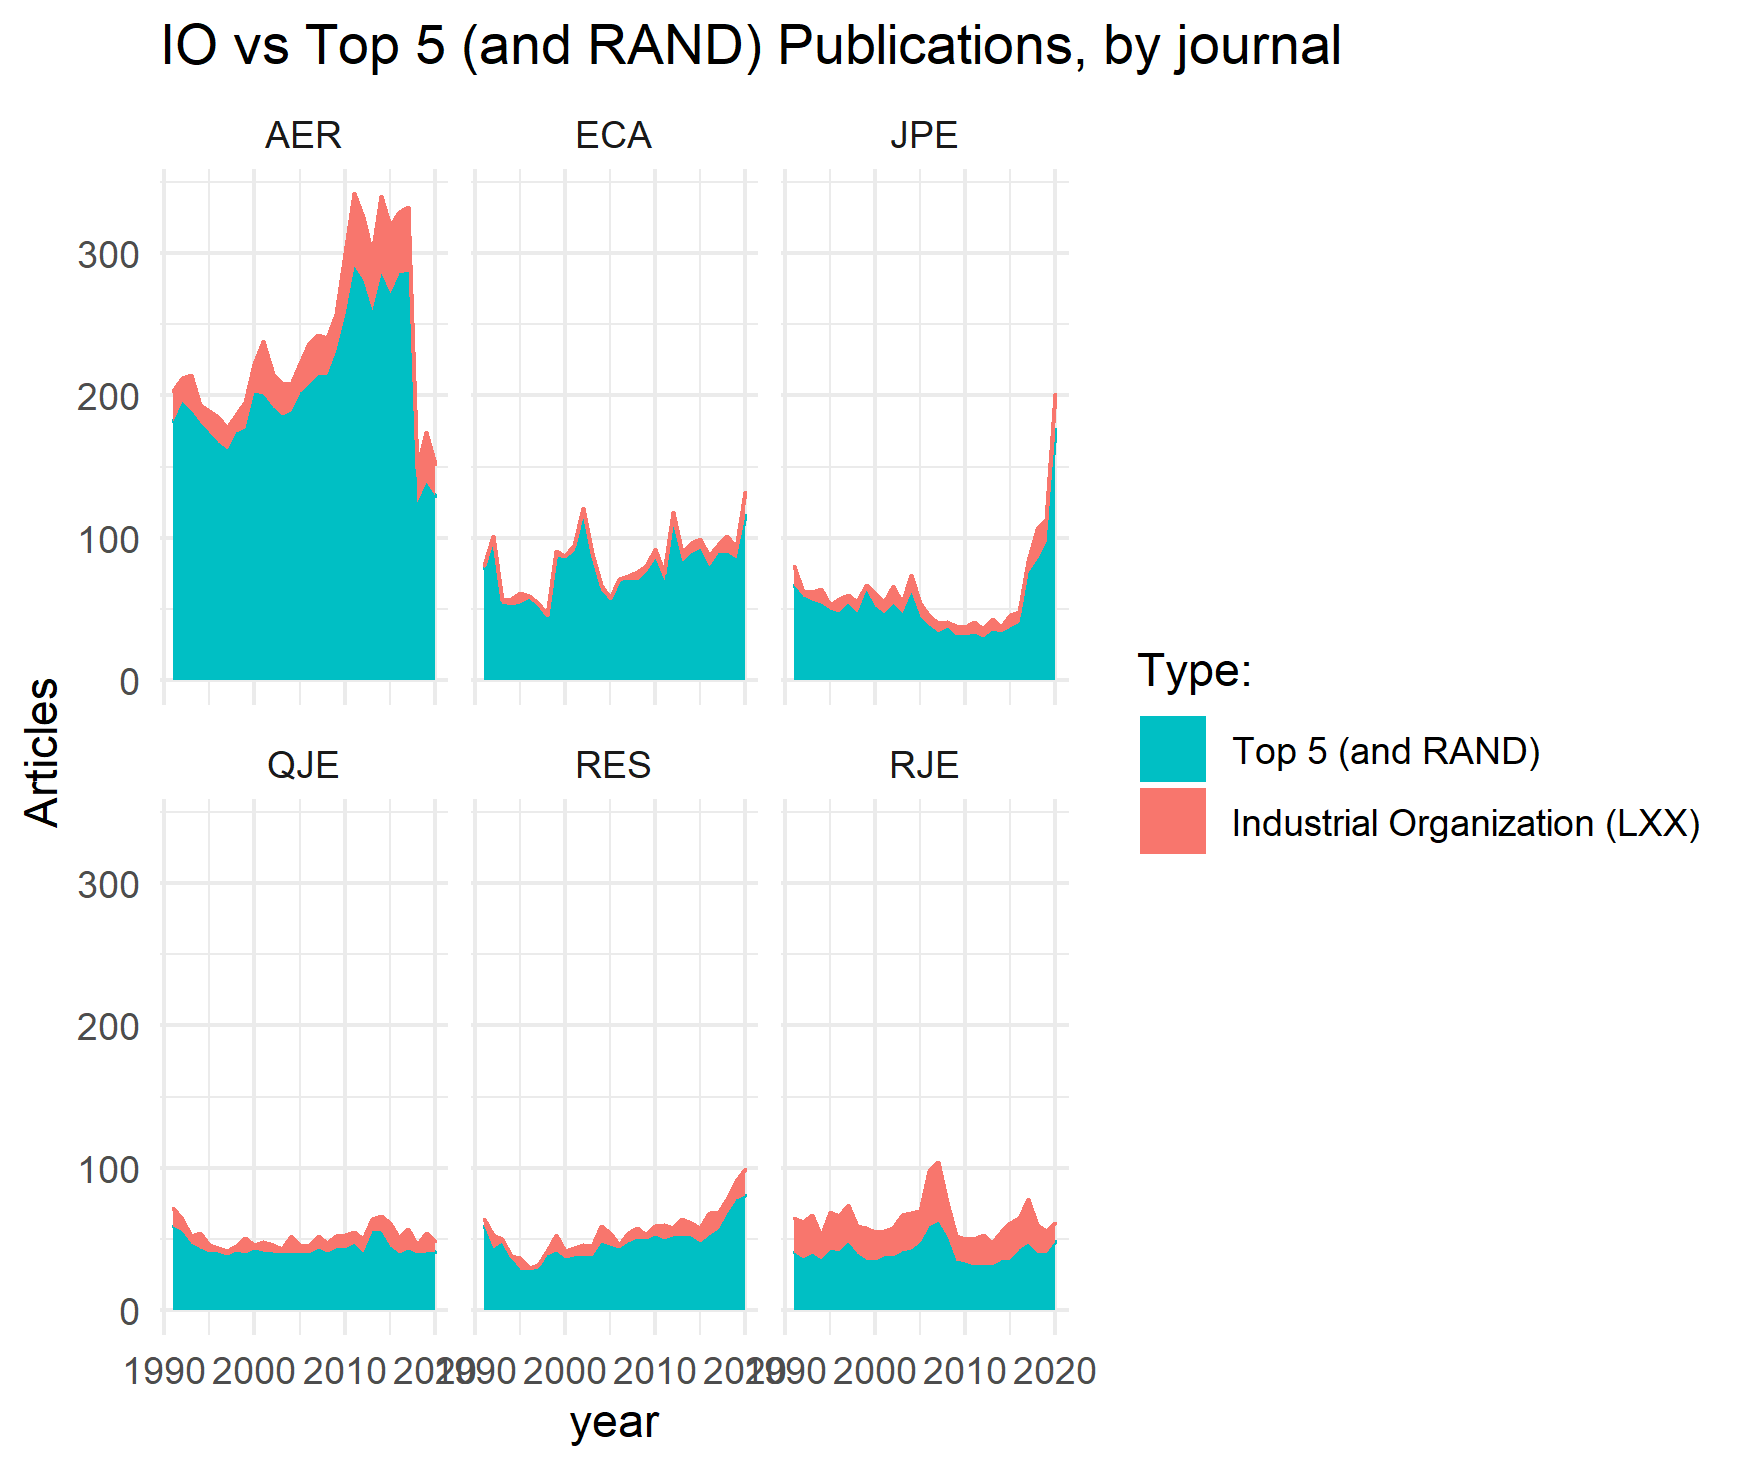
\includegraphics[width=\textwidth]{LXX-code-share-area-by-journal.png}
    \end{subfigure}
    \hfill
    \begin{subfigure}[!htbp]{0.49\textwidth}
        \centering
        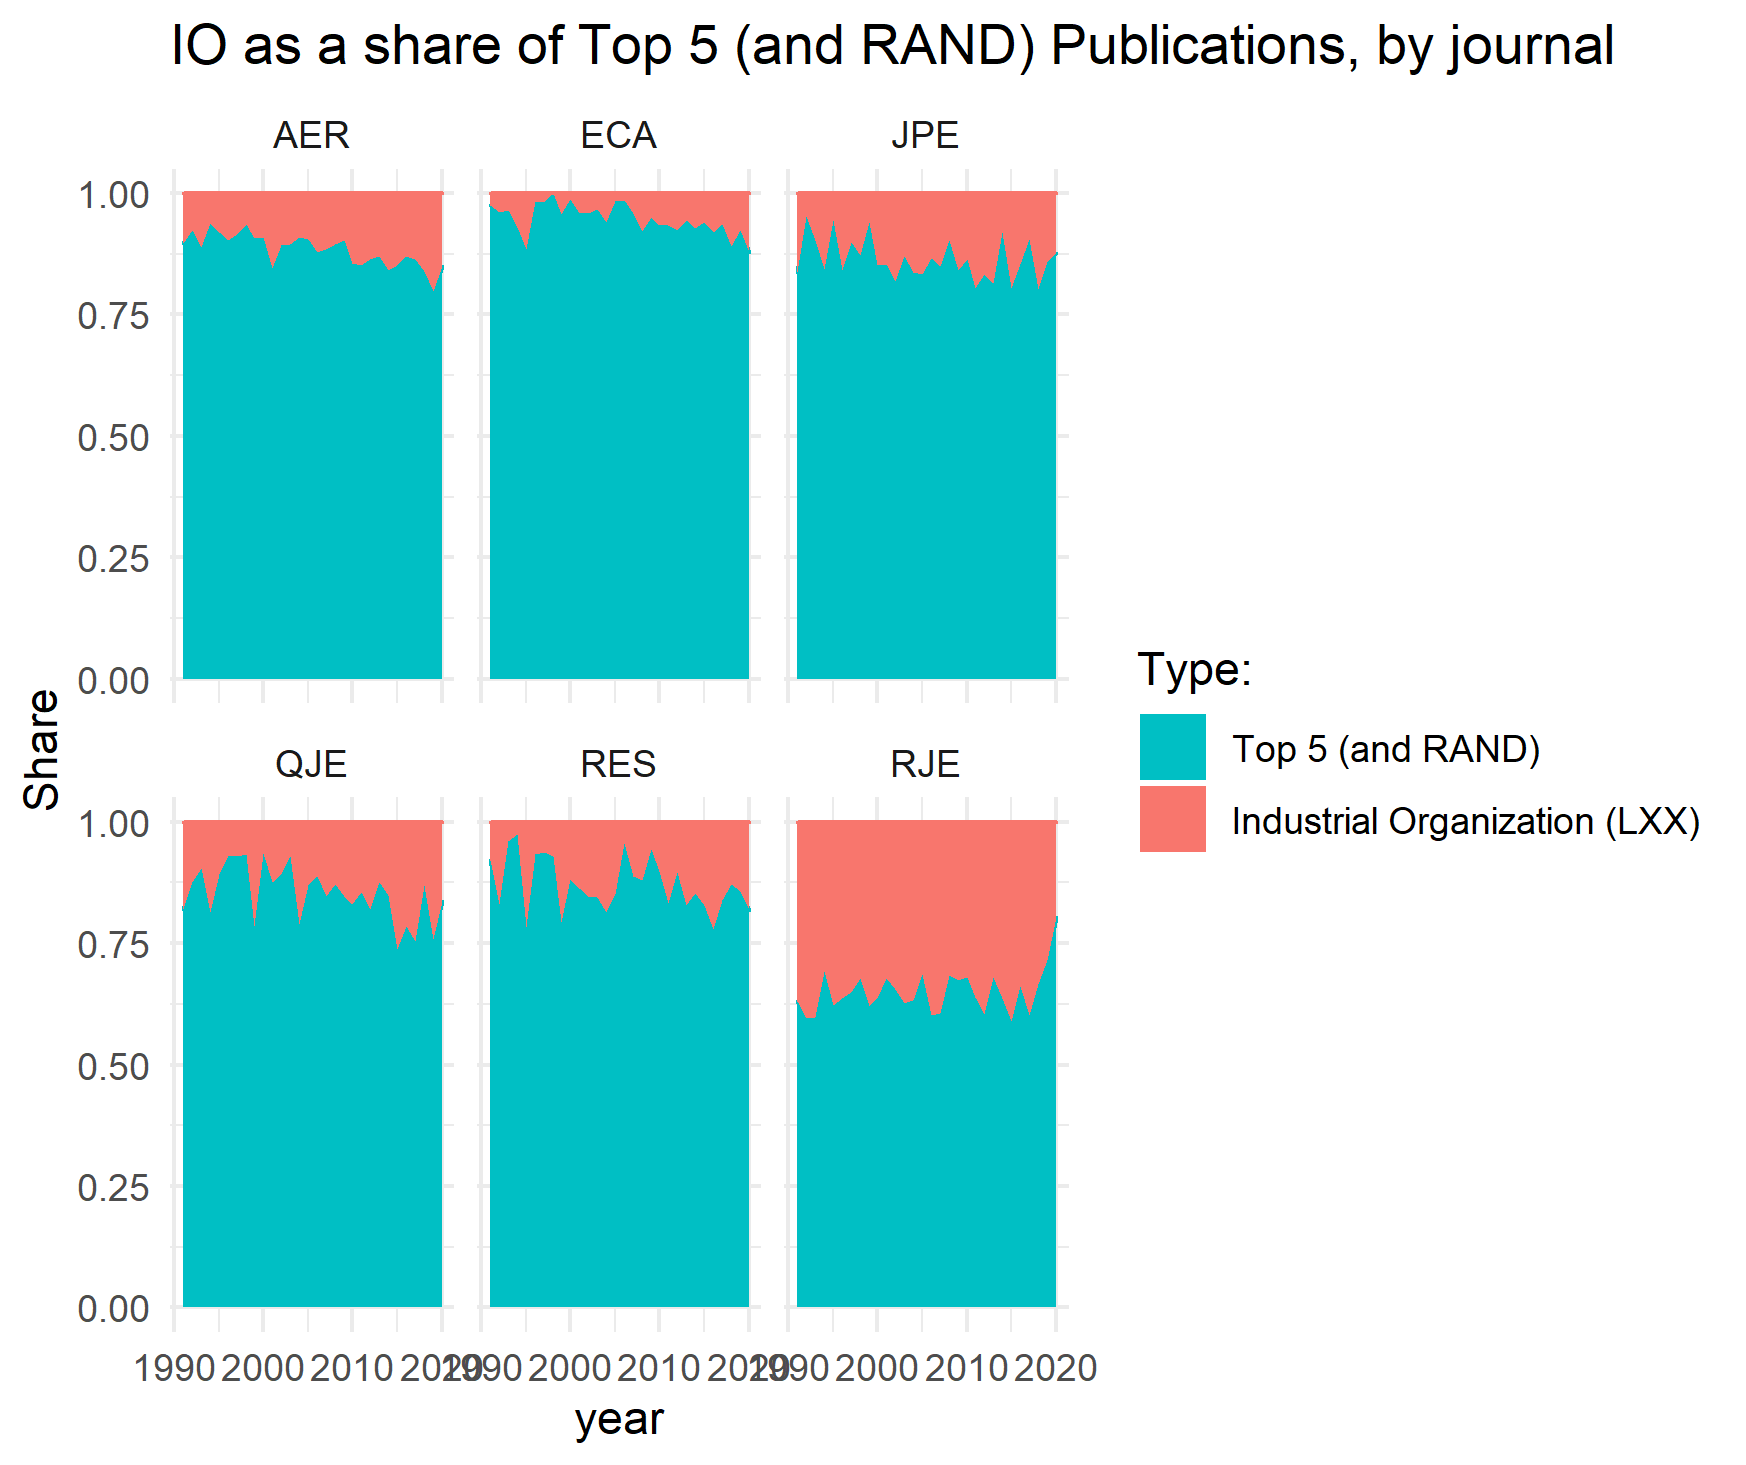
\includegraphics[width=\textwidth]{LXX-code-share-area-normalized-by-journal.png}
    \end{subfigure}
\end{figure}

\newpage

\section{The Role of Anti-Trust}

\begin{figure}
    \begin{subfigure}[!htbp]{0.49\textwidth}
        \centering
        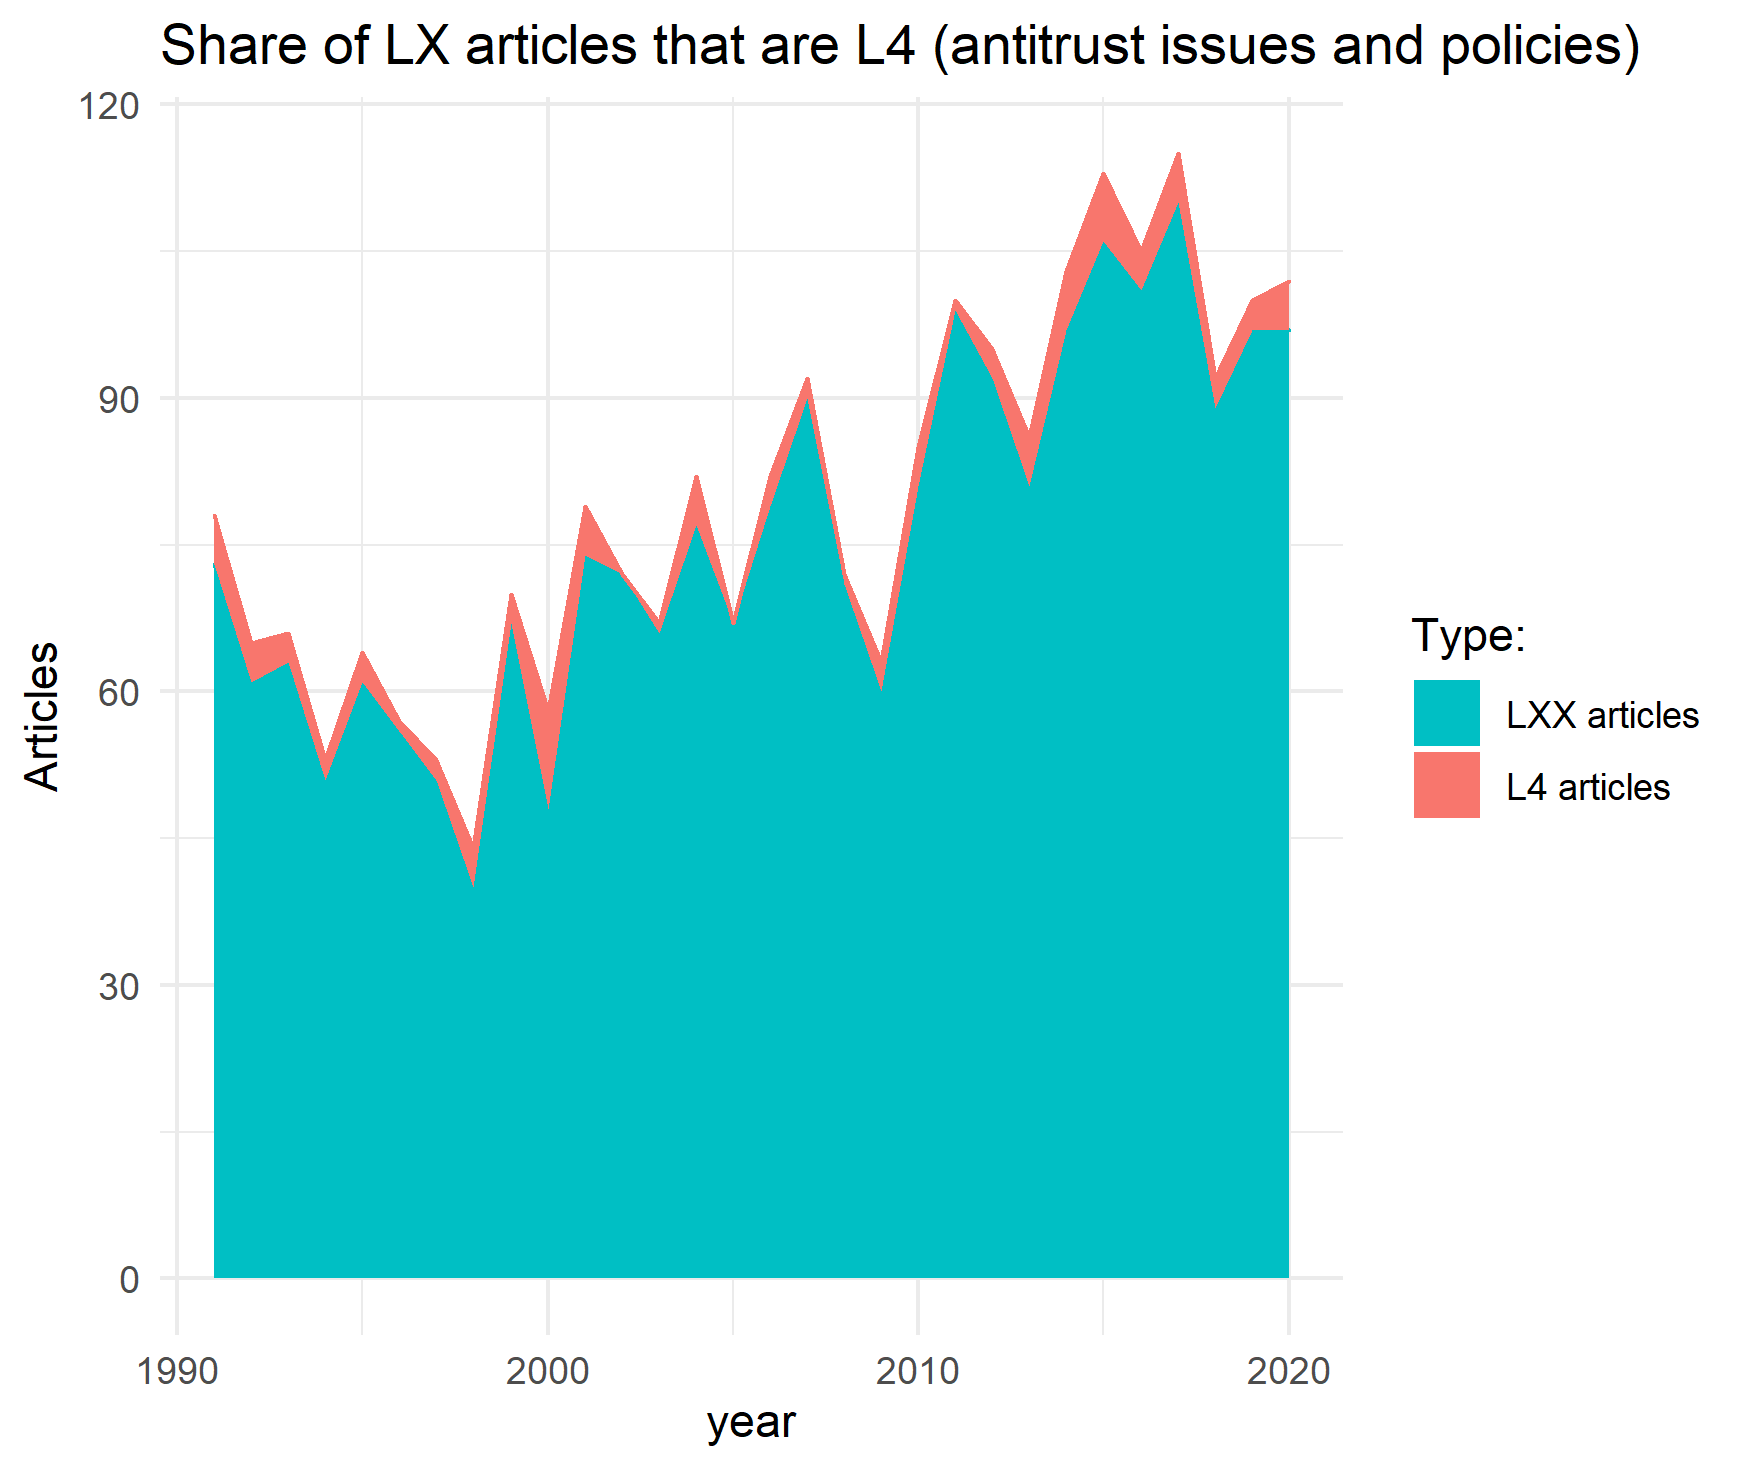
\includegraphics[width=\textwidth]{L4-vs-LXX.png}
    \end{subfigure}
    \hfill
    \begin{subfigure}[!htbp]{0.49\textwidth}
        \centering
        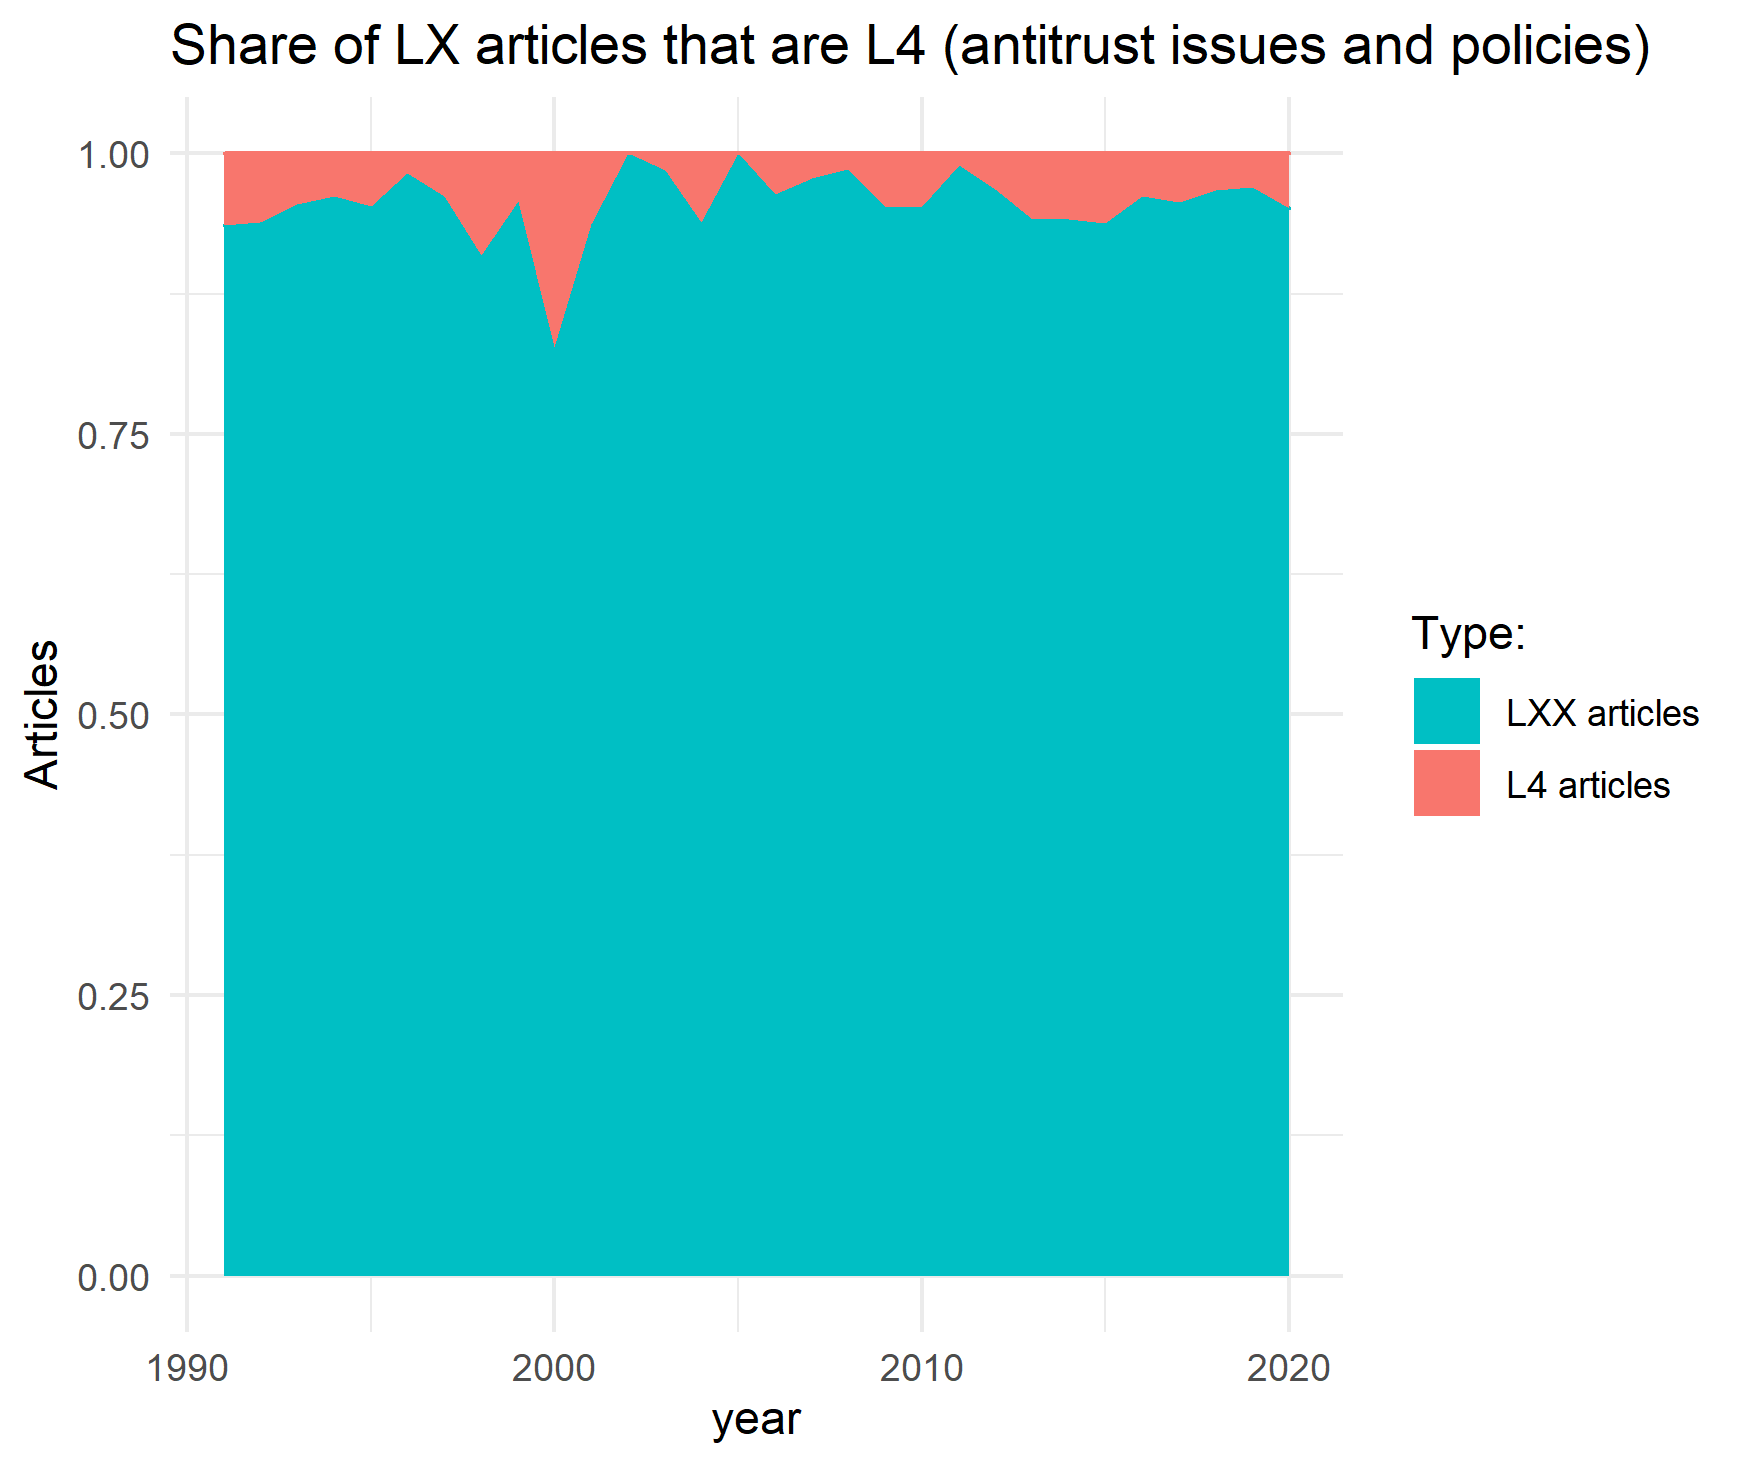
\includegraphics[width=\textwidth]{L4-vs-LXX-normalized.png}
    \end{subfigure}
\end{figure}


\begin{figure}
    \begin{subfigure}[!htbp]{0.49\textwidth}
        \centering
        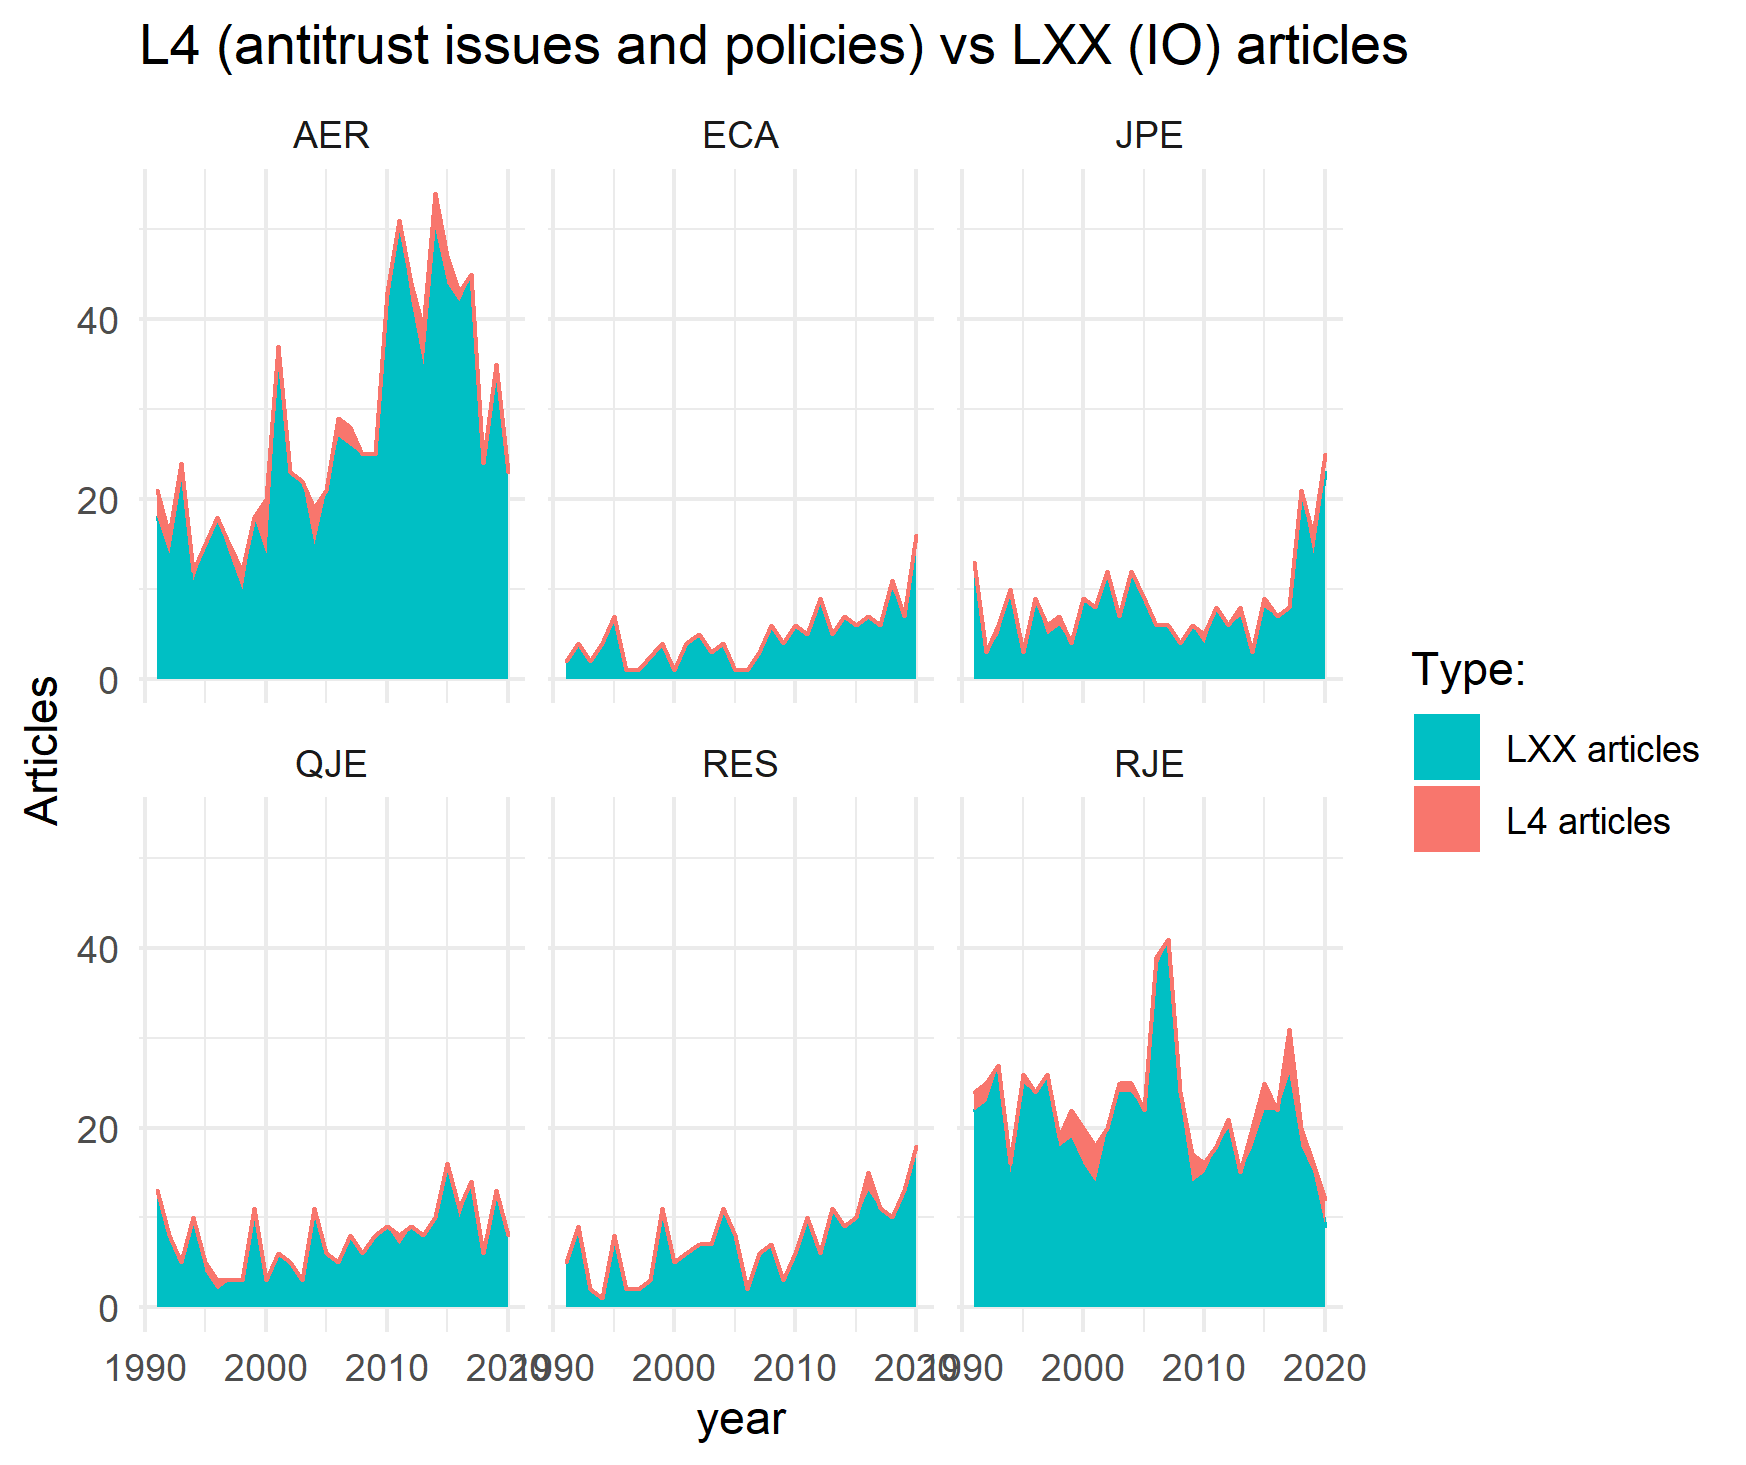
\includegraphics[width=\textwidth]{L4-vs-LXX-by-journal.png}
    \end{subfigure}
    \hfill
    \begin{subfigure}[!htbp]{0.49\textwidth}
        \centering
        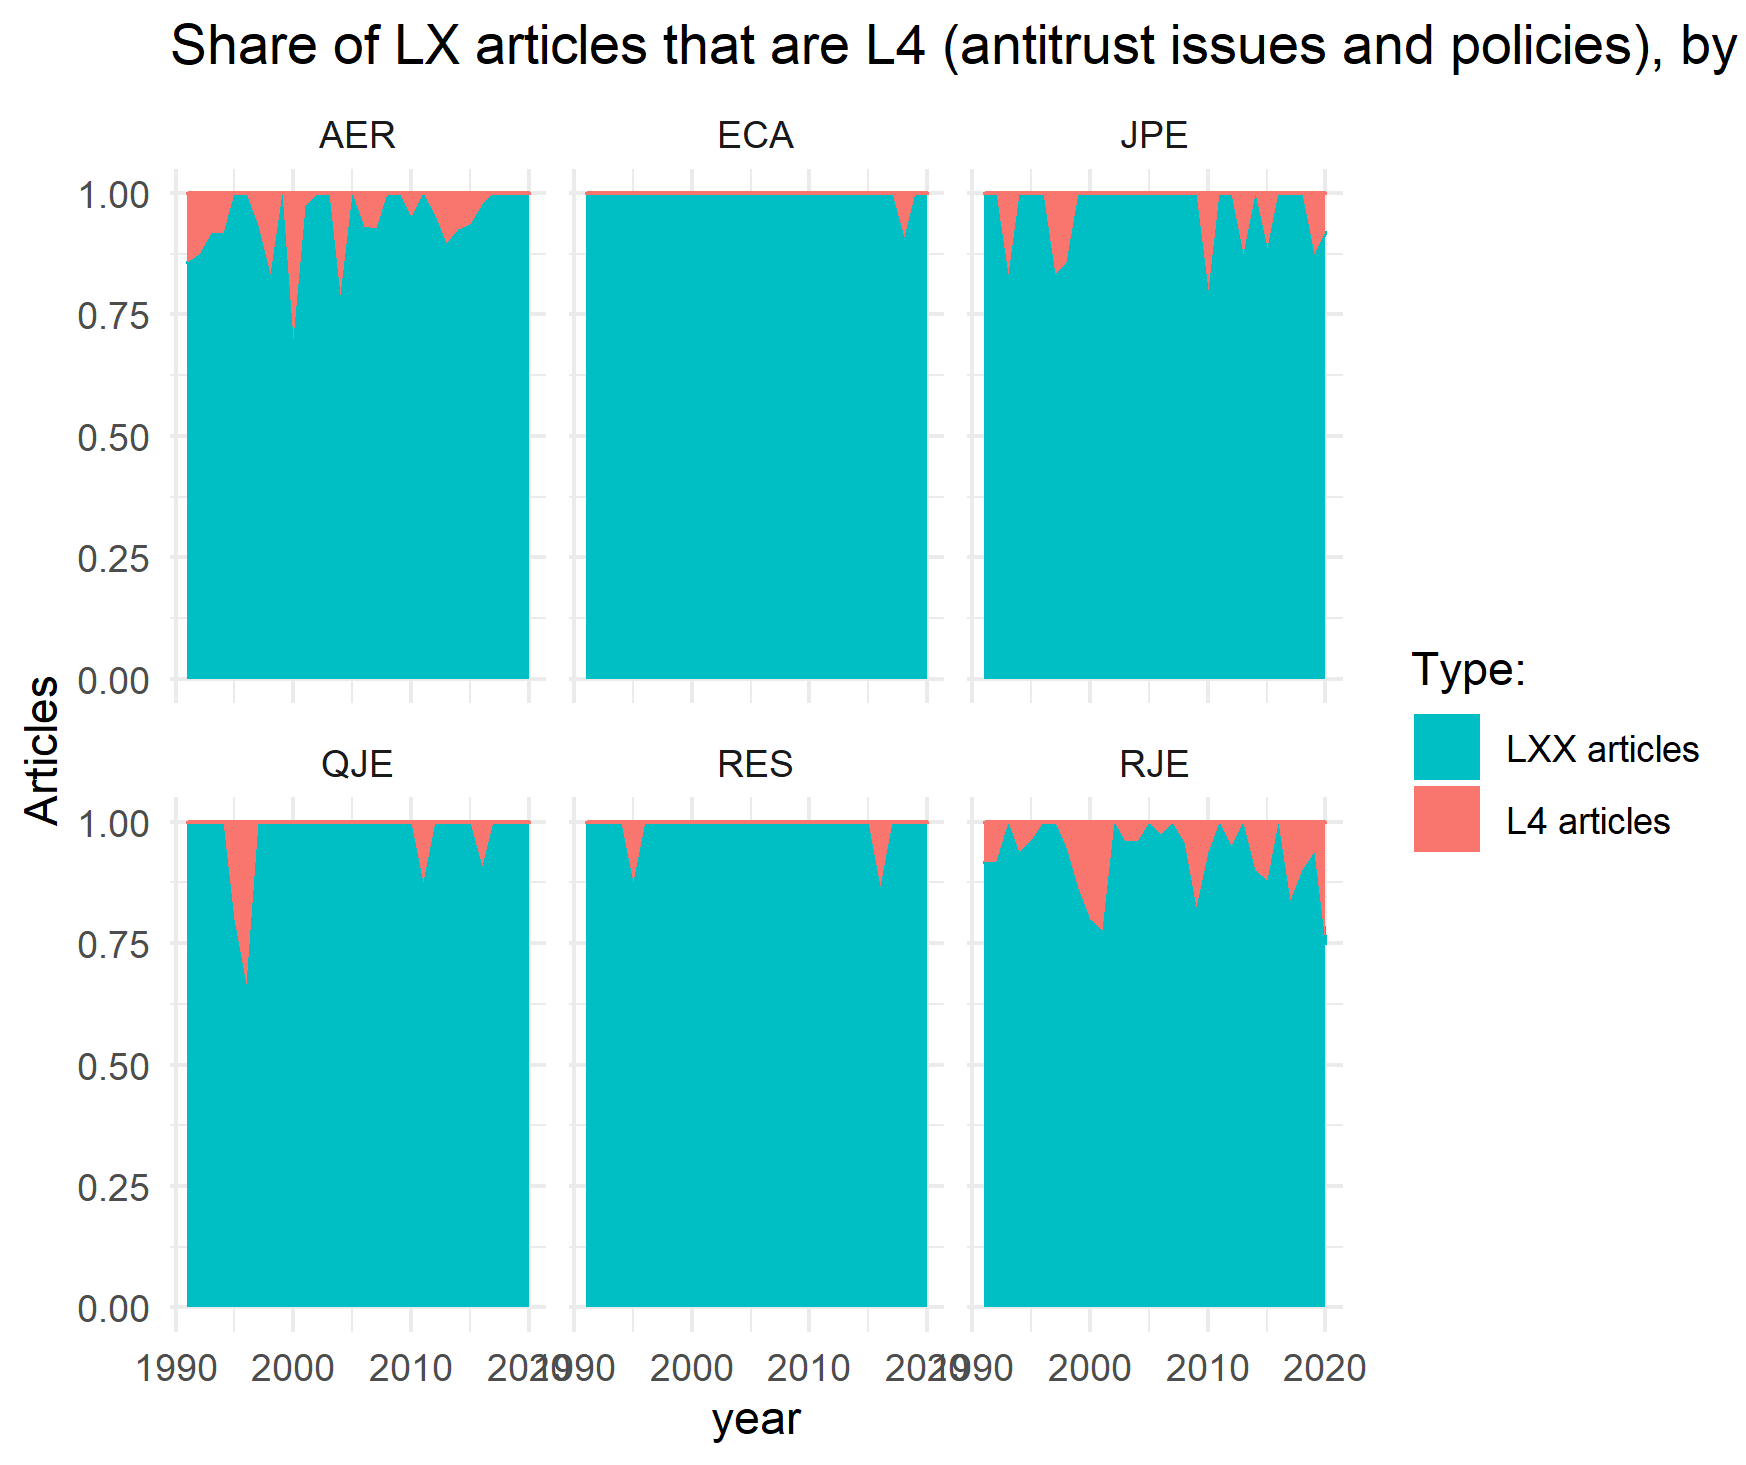
\includegraphics[width=\textwidth]{L4-vs-LXX-normalized-by_journal.png}
    \end{subfigure}
\end{figure}



\newpage

\begin{table}[!htbp] \centering 
    \caption{} 
    \label{} 

    \begin{adjustbox}{max width=\textwidth}
        \begin{tabular}{@{\extracolsep{5pt}} ccccccccccc} 
            \\[-1.8ex]\hline 
            \hline \\[-1.8ex]
            & \multicolumn{6}{c}{\textit{Abstract contains:}} & \multicolumn{4}{c}{\textit{JEL Code}} \\ 
          \cline{2-7} \cline{8-11} \\
            Publication & Anti Trust & Market Power & Anti Competitive & Monopoly & Merger & Cartel & L & K & L4 & K21 \\ 
            \hline \\[-1.8ex] 
            AER & 11 & 25 & 6 & 52 & 30 & 15 & 869 & 216 & 43 & 24 \\ 
            ECA & 1 & 8 & 1 & 22 & 4 & 3 & 154 & 20 & 1 & 7 \\ 
            JPE & 5 & 16 & 1 & 27 & 7 & 5 & 279 & 78 & 12 & 7 \\ 
            QJE & 1 & 12 & 1 & 25 & 8 & 0 & 239 & 60 & 4 & 0 \\ 
            RES & 2 & 9 & 1 & 52 & 5 & 2 & 228 & 39 & 3 & 1 \\ 
            RJE & 21 & 37 & 13 & 113 & 48 & 16 & 679 & 87 & 43 & 15 \\ 
            TOTAL & 41 & 107 & 23 & 291 & 102 & 41 & 2448 & 500 & 106 & 54 \\ 
            \hline \\[-1.8ex] 
        \end{tabular} 

          
    \end{adjustbox}
    
\end{table} 



\end{document}